\documentclass[twoside]{article}
\setlength{\oddsidemargin}{0.25 in}
\setlength{\evensidemargin}{-0.25 in}
\setlength{\topmargin}{-0.6 in}
\setlength{\textwidth}{6.5 in}
\setlength{\textheight}{8.5 in}
\setlength{\headsep}{0.75 in}
\setlength{\parindent}{0 in}
\setlength{\parskip}{0.1 in}

\usepackage{graphicx}
\usepackage{url}
\usepackage{multicol}
\usepackage{listings}

%
% The following commands sets up the lecnum (lecture number)
% counter and make various numbering schemes work relative
% to the lecture number.
%
\newcounter{lecnum}
\renewcommand{\thepage}{\thelecnum-\arabic{page}}
\renewcommand{\thesection}{\thelecnum.\arabic{section}}
\renewcommand{\theequation}{\thelecnum.\arabic{equation}}
\renewcommand{\thefigure}{\thelecnum.\arabic{figure}}
\renewcommand{\thetable}{\thelecnum.\arabic{table}}
\newcommand{\dnl}{\mbox{}\par}

%
% The following macro is used to generate the header.
%
\newcommand{\lecture}[4]{
  \pagestyle{myheadings}
  \thispagestyle{plain}
  \newpage
  \setcounter{lecnum}{#1}
  \setcounter{page}{1}
  \noindent
  \begin{center}
  \framebox{
     \vbox{\vspace{2mm}
   \hbox to 6.28in { {\bf CMPSCI~630~~~Systems
                       \hfill Fall 2014} }
      \vspace{4mm}
      \hbox to 6.28in { {\Large \hfill Lecture #1  \hfill} }
%       \hbox to 6.28in { {\Large \hfill Lecture #1: #2  \hfill} }
      \vspace{2mm}
      \hbox to 6.28in { {\it Lecturer: #3 \hfill Scribe: #4} }
     \vspace{2mm}}
  }
  \end{center}
  \markboth{Lecture #1: #2}{Lecture #1: #2}
  \vspace*{4mm}
}

%
% Convention for citations is authors' initials followed by the year.
% For example, to cite a paper by Leighton and Maggs you would type
% \cite{LM89}, and to cite a paper by Strassen you would type \cite{S69}.
% (To avoid bibliography problems, for now we redefine the \cite command.)
%
\renewcommand{\cite}[1]{[#1]}

% \input{epsf}

%Use this command for a figure; it puts a figure in wherever you want it.
%usage: \fig{NUMBER}{FIGURE-SIZE}{CAPTION}{FILENAME}
\newcommand{\fig}[4]{
           \vspace{0.2 in}
           \setlength{\epsfxsize}{#2}
           \centerline{\epsfbox{#4}}
           \begin{center}
           Figure \thelecnum.#1:~#3
           \end{center}
   }

% Use these for theorems, lemmas, proofs, etc.
\newtheorem{theorem}{Theorem}[lecnum]
\newtheorem{lemma}[theorem]{Lemma}
\newtheorem{proposition}[theorem]{Proposition}
\newtheorem{claim}[theorem]{Claim}
\newtheorem{corollary}[theorem]{Corollary}
\newtheorem{definition}[theorem]{Definition}
\newenvironment{proof}{{\bf Proof:}}{\hfill\rule{2mm}{2mm}}

% Some useful equation alignment commands, borrowed from TeX
\makeatletter
\def\eqalign#1{\,\vcenter{\openup\jot\m@th
 \ialign{\strut\hfil$\displaystyle{##}$&$\displaystyle{{}##}$\hfil
     \crcr#1\crcr}}\,}
\def\eqalignno#1{\displ@y \tabskip\@centering
 \halign to\displaywidth{\hfil$\displaystyle{##}$\tabskip\z@skip
   &$\displaystyle{{}##}$\hfil\tabskip\@centering
   &\llap{$##$}\tabskip\z@skip\crcr
   #1\crcr}}
\def\leqalignno#1{\displ@y \tabskip\@centering
 \halign to\displaywidth{\hfil$\displaystyle{##}$\tabskip\z@skip
   &$\displaystyle{{}##}$\hfil\tabskip\@centering
   &\kern-\displaywidth\rlap{$##$}\tabskip\displaywidth\crcr
   #1\crcr}}
\makeatother

% **** IF YOU WANT TO DEFINE ADDITIONAL MACROS FOR YOURSELF, PUT THEM HERE:



% Some general latex examples and examples making use of the
% macros follow.

\begin{document}

%FILL IN THE RIGHT INFO.
%\lecture{**LECTURE-NUMBER**}{**DATE**}{**LECTURER**}{**SCRIBE**}
\lecture{8}{September 25}{Emery Berger}{Amee Trivedi}


\section*{Lecture Summary}
%\section{Summary}
\begin{itemize}
	\item Synchronization
	\item D-Threads
	\item THE system design
\end{itemize}

\section{Synchronization}
Non-determinism is the behaviour when the result of each run of a program is different. Eg:
 If there are 2 threads t1 and t2 such that:

\begin{lstlisting}
	t1			t2
      a = 1		      a = 2

\end{lstlisting}

and if a is global, the o/p can be 1 or 2

Now,
\begin{lstlisting}
	  t1			t2
  			      a = 2
				.
    	a = 1			.
				.(after lapse of a day)
			      print a
\end{lstlisting}

The results would be 1 or undefined in the case of C/C++ because C/C++ will get the value from "thin air".
Access from RAM is in chunks of memory called cachelines. Protocol MESI takes care of cache-coherence.
M -> Modified
E -> Exclusive
S -> Shared
I -> Invalid

\begin{figure}[ht!]
\center
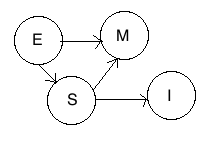
\includegraphics[width=40mm]{MESI.png}
\caption{ MESI Transition states \label{MESI}}
\end{figure}

AMD added O for Ownership and made it MOESI.

\subsection{False Sharing}

\begin{lstlisting}[language=C]
		int a = 0
		int b = 0

   	  t1			  t2
	a = 1			b = 2
	for(...)		for(...)
	{ 			{
	... 			...
	a++ 			b++
	} 			}
\end{lstlisting}


The resultant values of a and b depend on wether they are in the same cache line or different.
If t2 is executed first followed by t1 and they are in the same cacheline then the copy of t1 is always discarded. This is called false sharing. This happens though the values of a and b are logically unshared but are physically shared. This can result in cache line pingponging.

To implement cache coherence Snoopy cache and Directory based protocols are used among other techniques.

\subsection{Sequential V/s Concurrency}


\begin{enumerate}
	\item a=1
	\item b=2
	\item spawn f(a)
	\item spawn f(b)
	\item sync
	\item print a
\end{enumerate}

The flow diagram would be as  follows:

\begin{figure}[ht!]
\centering
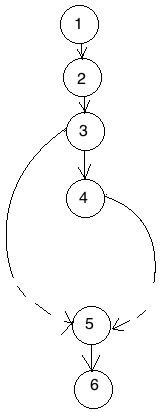
\includegraphics[width=24mm]{seq_con.png}
\caption{Flow diagramn \label{Flow diagram}}
\end{figure}

Inst 3 and Inst 4 result in 2 threads but inst 5 results in merge of flow.

For synchronization in a "co-operative sync process" model we need atomic reads and writes. Atomic operation is defined as an indivisible operation based on the word size of the system.

If there are regions in code that should be accessed only by a single thread at a given time then the region is called critical region. Locks are used to ensure that only one thread executes in a critical region. 

Code to lock a resource would look as below:

\begin{lstlisting}[language=C]
	TEST_AND_SET(l)
	if (l == 0) {
	  l = 1;
	  return true;
	}
	return false;
\end{lstlisting}

So, a thread code for locking a resource would look like:

\begin{lstlisting}[language=C]
lock(l):
while (true) {
  r = TEST_AND_SET(l);
  if (r)
    return;
} \\This mecahnism of locking is called Spin lock
\end{lstlisting}

or

\begin{lstlisting}[language=C]
lock(l):
while (true) {
	...
} 
sleep();
sched_yield() \\ This mechanism is called spin and block lock

\end{lstlisting}



To unlock all you do is reset 1 to 0, so, the code looks like:

\begin{lstlisting}[language=C]
unlock(l):
{
  l = 0;
}
\end{lstlisting}

\section{D-threads}

Removes race condition by updating the memory to global memory in a specific order. There are 2 ways of analysis, static and dynamic.

\subsection{Static Analysis}
\begin{itemize}
	\item It sees program instruction
	\item Reports lots of false alarms(cases where it detects race conditions but only a few are true)
	\item It has high coverage
\end{itemize}

\subsection{Dynamic Analysis}
\begin{itemize}
	\item It has lower coverage
	\item Reports things that are only real
	\item t misses a lot of scenarios which can result on a different system/environment/load conditions
\end{itemize}

\section{THE}
\begin{itemize}
	\item Introduced layered approach, which is currently used in networking stack
	\item This approach is called "Separation of concerns"
	\item Advantages of layered approaches are:
		\begin{itemize}
			\item Easy to test things independently
			\item Composable
			\item Modular
		\end{itemize}
	\item So, the system aproach went from Monolithic to layered approach
\end{itemize}
Then came microkernels and the war between MINIX and LINUX.

\end{document}
